\setcounter{page}{1}

\section{文字排版}
\subsection{插入文字}
在新的阅读视图中阅读更加容易。可以折叠文档某些部分并关注所需文本。如果在达到结尾处之前需要停止读取,Word 会记住您的停止位置 - 即使在另一个设备上。视频提供了功能强大的方法帮助您证明您的观点。当您单击联机视频时,可以在想要添加的视频的嵌入代码中进行粘贴。您也可以键入一个关键字以联机搜索最适合您的文档的视频。\cite{a2021b}
\par 为使您的文档具有专业外观,Word 提供了页眉、页脚、封面和文本框设计,这些设计可互为补充。例如,您可以添加匹配的封面、页眉和提要栏。单击“插入”,然后从不同库中选择所需元素。主题和样式也有助于文档保持协调。当您单击设计并选择新的主题时,图片、图表或 SmartArt 图形将会更改以匹配新的主题。当应用样式时,您的标题会进行更改以匹配新的主题。


\subsection{列出清单}
\par 本系统实现以下功能模块:
\begin{itemize}
    \item[1.] 功能1
    \item[2.] 功能2
    \item[3.] 功能3
\end{itemize}
\section{公式排版}
\subsection{插入公式}
\[
    3/8 \qquad \frac{3}{8}
    \qquad \tfrac{3}{8}
\]

\[
    a^2  = b^2 + c^2
\]

\section{图片排版}
\subsection{插入图片}
\subsubsection{单栏插入}

\begin{figure}[H]
    \centering
    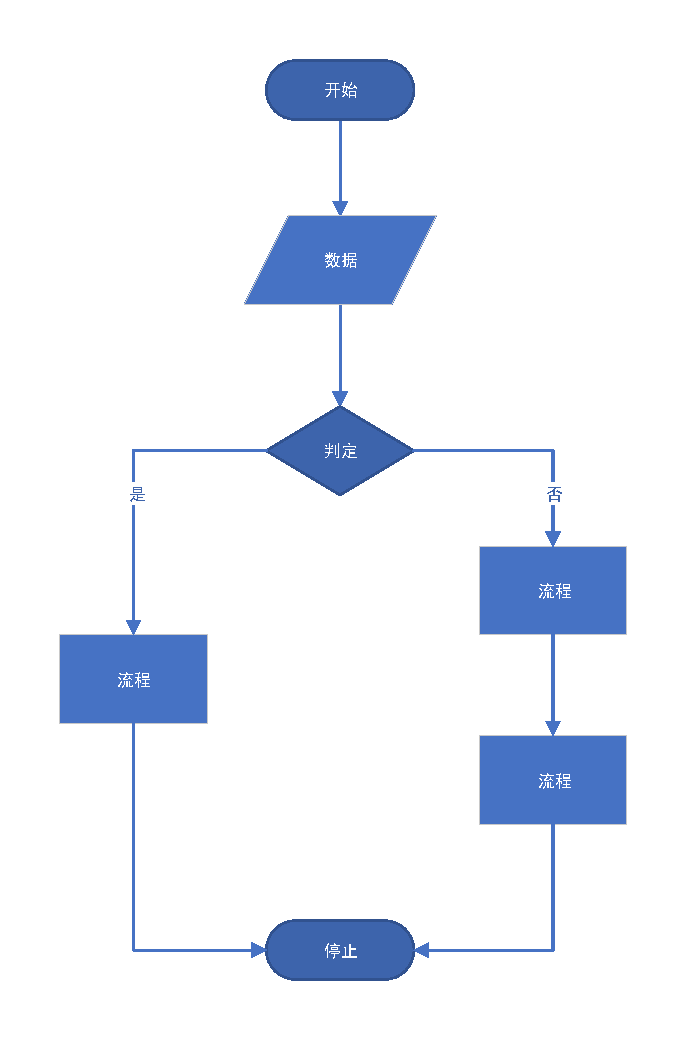
\includegraphics [width=0.6\textwidth]{测试.pdf}
    \caption{测试}
\end{figure}



\subsubsection{双栏插入}


\begin{figure}[H]
    \centering
    \begin{minipage}[c]{0.5\textwidth}
        \centering
        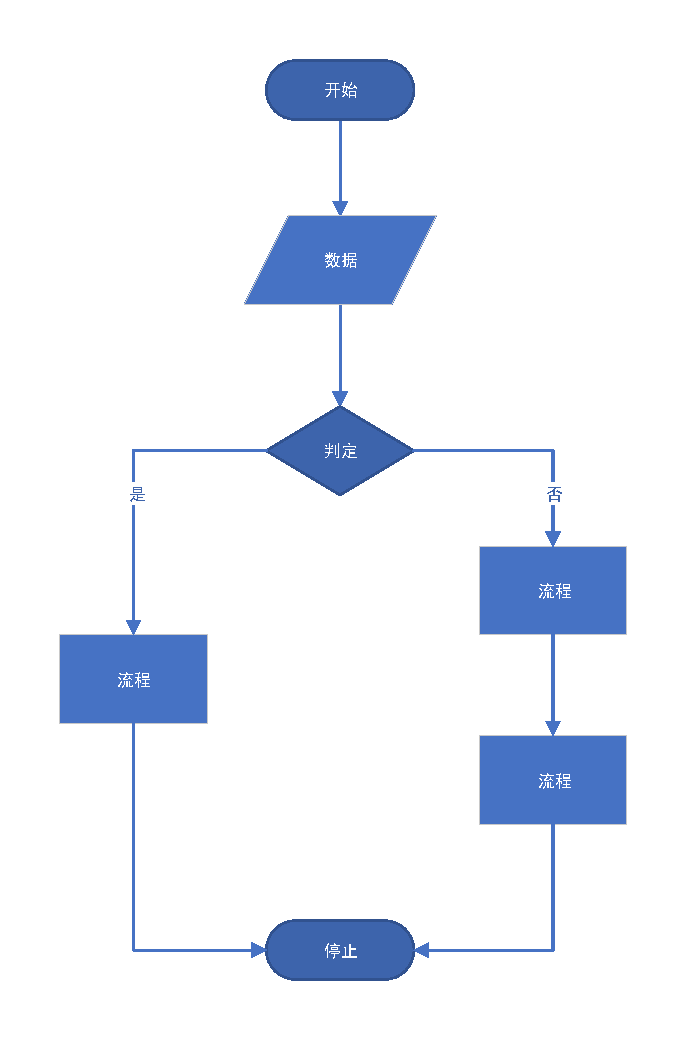
\includegraphics[width=1\textwidth]{测试.pdf}
        \caption{测试}
    \end{minipage}%
    \begin{minipage}[c]{0.5\textwidth}
        \centering
        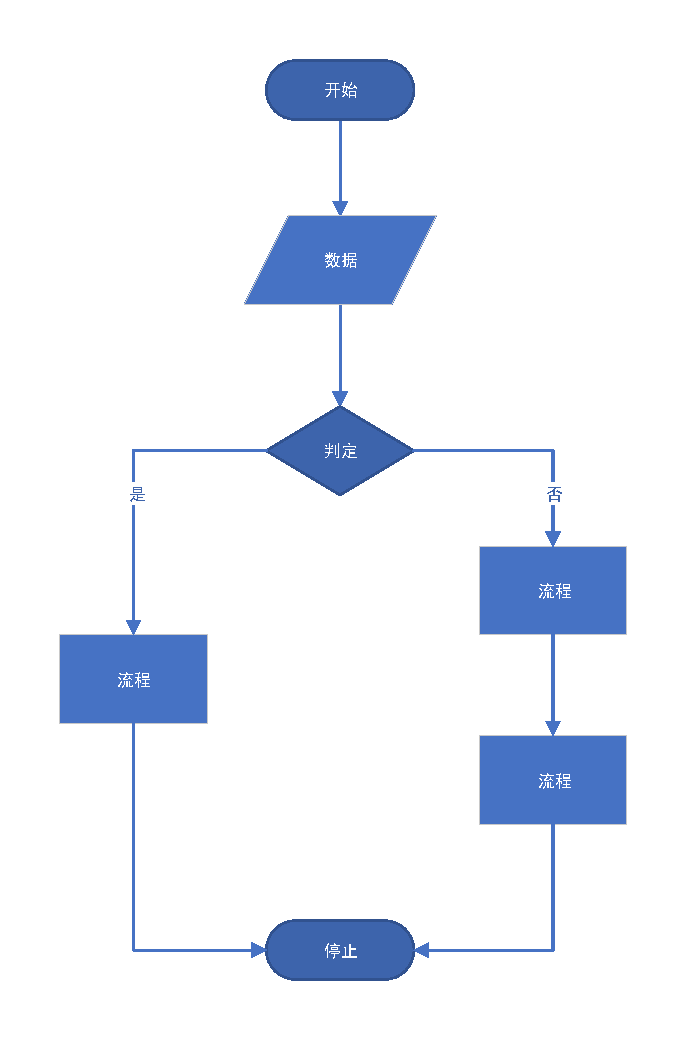
\includegraphics[width=1\textwidth]{测试.pdf}
        \caption{测试.pdf}
    \end{minipage}
\end{figure}

\section{表格排版}
\subsection{普通表格}
\begin{table}[H]
    \centering
    \caption{简单表格}
    \label{tab:1}
    \begin{tabular}{|l|c|r|}
        \hline
        我是 & 一只 & 普通 \\
        \hline
        的   & 表格 & 呀   \\
        \hline
    \end{tabular}
\end{table}
\subsection{三线表}

\begin{table}[htbp]
    \centering
    \caption{探测器转换系数和电压脉冲幅度对比}
    \begin{tabular}{ccc}
        \toprule
                                         & 能量电荷转换系数                                              & 输出脉冲幅度                                           \\
        \midrule
        \multicolumn{1}{l}{电离室}       & \multicolumn{1}{r} {$3 \times 10^4$ 电子对/MeV }              & \multicolumn{1}{r}  {$5 \times 10^{-4}$ V/MeV }        \\
        \multicolumn{1}{l}{正比计数器}   & \multicolumn{1}{r} {$3 \times 10^4 \bar{A}$  电子离子对/MeV } & \multicolumn{1}{r}  {$5 \times 10^{-4}\bar{A}$ V/MeV } \\
        \multicolumn{1}{l}{闪烁探测器}   & \multicolumn{1}{r} {$300 \bar{M}$   电子/MeV}                 & \multicolumn{1}{r}  {$5 \times 10^{-6}\bar{M}$ V/MeV } \\
        \multicolumn{1}{l}{半导体探测器} & \multicolumn{1}{r}  { $3 \times 10^5$   电子空穴对/MeV}       & \multicolumn{1}{r}  {$5 \times 10^{-3}$ V/MeV }        \\
        \bottomrule
    \end{tabular}
\end{table}
\section{代码排版}
\subsection{SQL语句}

\begin{lstlisting}[language=SQL]
--------------------------------------------------------
--  DDL for Table T_STUDENT
--------------------------------------------------------

  CREATE TABLE "XX" 
   (	"XX" VARCHAR2(20 BYTE), 
	"XX1" VARCHAR2(20 BYTE), 
	"XX2" VARCHAR2(20 BYTE), 
	"XX3" VARCHAR2(20 BYTE), 
	"XX4" VARCHAR2(20 BYTE), 
	"XX5" VARCHAR2(20 BYTE), 
	"XX6" VARCHAR2(20 BYTE)
   );
--------------------------------------------------------
--  Constraints for Table T_STUDENT
--------------------------------------------------------

  ALTER TABLE "XX" ADD CONSTRAINT "T_STUDENT_PK" PRIMARY KEY ("XX1");
  ALTER TABLE "XX" MODIFY ("XX1" NOT NULL ENABLE);
  ALTER TABLE "SXX" MODIFY ("XX2" NOT NULL ENABLE);

\end{lstlisting}
\subsection{C语言}
\lstinputlisting[language=C]{code/c-main}
\subsection{JAVA}
\lstinputlisting[language=JAVA]{code/java-HelloWorld}



\newpage
\section{总结}
使用在需要位置出现的新按钮在 Word 中保存时间。若要更改图片适应文档的方式,请单击该图片,图片旁边将会显示布局选项按钮。当处理表格时,单击要添加行或列的位置,然后单击加号。在新的阅读视图中阅读更加容易。可以折叠文档某些部分并关注所需文本。如果在达到结尾处之前需要停止读取,Word 会记住您的停止位置 - 即使在另一个设备上。
\par 视频提供了功能强大的方法帮助您证明您的观点。当您单击联机视频时,可以在想要添加的视频的嵌入代码中进行粘贴。您也可以键入一个关键字以联机搜索最适合您的文档的视频。为使您的文档具有专业外观,Word 提供了页眉、页脚、封面和文本框设计,这些设计可互为补充。例如,您可以添加匹配的封面、页眉和提要栏。单击“插入”,然后从不同库中选择所需元素。
